\documentclass[11pt,a4paper]{article}

\usepackage{dirtree}

\usepackage{amsmath}
\usepackage{amsfonts}
\usepackage{amssymb}
\usepackage{amsthm}

%Arbritary font sizes
\usepackage{lmodern}% http://ctan.org/pkg/lm

\usepackage{tikz}
%Some Graphics / Flowcharts etc.
\tikzset{rounded/.style={rounded corners}}

\usepackage{listings}
\lstset{basicstyle=\footnotesize\ttfamily,breaklines=true}

%Margin setup
\usepackage[top=2cm, bottom=3cm, left=3cm, right=3cm]{geometry}

%Line spread
\linespread{1.3}

%FloatBarriers avoid usage 
\usepackage{placeins}

%show margin for development
%\usepackage{showframe}
%\overfullrule=2cm

%Fonts
\usepackage{xltxtra,fontspec,xunicode}

%for math
%\usepackage{cmbright}
%\usepackage{XCharter}
%\usepackage[T1]{fontenc}

\usepackage[bitstream-charter]{mathdesign}
\usepackage[T1]{fontenc}
\DeclareTextCommand{\nobreakspace}{T1}{\leavevmode\nobreak\ }
\usepackage[scaled]{berasans}
\usepackage{beramono}
%\setkomafont{disposition}{\normalcolor\bfseries} % get rid of sans section headings

%\usepackage{todonotes}
\usepackage{booktabs}

\usepackage{float}

%sidecaptions
\usepackage{sidecap}

%used for formatting currency
\usepackage{siunitx}
\usepackage{eurosym}

\usepackage{graphicx}
\graphicspath{{graphics/}}

%% comment out if you like svg
\usepackage{svg}

%\svgpath{{graphics/}{graphics/inkscape/}}

%Used to create space after custom commands only if suitable
\usepackage{xspace}

%Control of captions and subcaptions
\usepackage[format=plain]{caption}
\usepackage[font=footnotesize]{subcaption}

\captionsetup[figure]{font=footnotesize,justification=raggedright}
\captionsetup[table]{font=footnotesize,justification=raggedright}

%Bibliography
\usepackage[sorting=none,citestyle=numeric,backend=biber]{biblatex}
\bibliography{Bibliography}

%Center verbatim environments for config file etc. presentation
\usepackage{fancyvrb}

% from : https://www.rhizobia.co.nz/latex/thesis
\hfuzz2pt % Don't bother to report over-full boxes if over-edge is < 2pt   

%Spacing between page and footnotes
\addtolength{\skip\footins}{2pc plus 5pt}
\setlength{\footnotesep}{1pc}

%Set footnotes in italics to distinguish from figure captions
\usepackage[flushmargin]{footmisc}
\renewcommand*{\footnotelayout}{\itshape}

%Consistent Indentation between TOC and LOF/LOT
\usepackage[titles]{tocloft}
\cftsetindents{figure}{0em}{3.5em}
\cftsetindents{table}{0em}{3.5em}


%hyperlinks (for citations)
\usepackage[hidelinks]{hyperref}
%use same font for urls
\urlstyle{same}

%Pseudocode listings
\usepackage{algorithm}
\usepackage{algpseudocode}


\theoremstyle{definition}
\newtheorem{definition}{Definition}

%Time
\usepackage[nodayofweek,level]{datetime}

\author{My Ky Huynh}
\title{Seurat Based scRNA-seq Snakemake Pipeline Documentation}

\newtheorem{hypothesis}{Hypothesis}

\begin{document}
	
	\pagenumbering{roman}
	
	\begin{titlepage}
	\begin{center}
		\vspace*{1cm}
		\Huge
		\makeatletter
		\textbf{\@title}
		\makeatother
		\vspace{1.5cm}
		
		\LARGE
		\makeatletter
		\textbf{\@author}
		\makeatother
		\vfill
		
		\vspace{0.8cm}
		
	\end{center}
\end{titlepage}
	
	\setcounter{page}{2}
	
%	\input{sections/ack}
	
%	\newpage
%	\input{Abstract}
	
	\newpage
	\tableofcontents
	
	\newpage
	
	\pagenumbering{arabic}
	
	\section{Introduction}
\label{section:intro}
This is the documentation for our Seurat based scRNA-seq pipeline with Snakemake.
The goal of this project was to automatize as many steps as possible.
There are a few points in the pipeline run where the pipeline will stop and throw an error, so you can take a look at a plot and choose a value for a function, e.g. given at the rule \textit{mt\_p1} an error will be thrown which tells you to look at a plot to choose at what percentage you want to filter the mitochondrial reads. However, it is possible to completely skip these error throws by filling in every value at the beginning. More on this in the workflow section. \textbf{The pipeline currently only accepts 10X Cellranger output folders as input.}

\subsection{Used R Packages}
The pipeline uses the R packages Seurat, DoubletFinder, seuratHelper and ShinyCell as main analysis packages.

\subsection{Pipeline Directory Structures}
\begin{minipage}{0.35\textwidth}
	\dirtree{%
		.1 path/to/scRNAseq\_Pipeline.
		.2 configfiles.
		.2 data.
		.2 dependencies.
		.2 documentation.
		.2 envs.
		.3 HHU\_HPC.
		.3 netAccess.
		.2 errorMessage.
		.2 scripts.
		.2 snakemakeScripts.
		.3 cluster.
		.2 workDirectory.
	}
\end{minipage}\hfill
\begin{minipage}{0.55\textwidth}
	\dirtree{%
	.1 \textbf{Folder applications}.
	.1 contains configfiles for analysis.
	.1 contains datasets.
	.1 packages for manual installation.
	.1 documentation.
	.1 conda envs.
	.1 for HHU HPC.
	.1 for internet access \& no restrictions.
	.1 contains \textbf{MissingInputError} texts .
	.1 contains R scripts.
	.1 contains scripts for pipeline config.
	.1 contains configs for on HHU HPC cluster.
	.1 contains an instruction .txt.
}
\end{minipage}

\subsection{Project Directory Structures}
\begin{minipage}{0.45\textwidth}
	\dirtree{%
		.1 path2/two/pipeline\_project\_output.
		.2 clusterLogs.
		.2 csv.
		.2 logs.
		.2 plot.
		.2 outputs.
		.2 shinyApp.
		.2 workDirectory.
	}
\end{minipage}\hfill
\begin{minipage}{0.45\textwidth}
	\dirtree{%
		.1 \textbf{Folder applications}.
		.1 logs created by cluster.
		.1 csv outputs.
		.1 snakemake logs.
		.1 plot outputs.
		.1 pipeline output .rds files.
		.1 shiny app.
		.1 contains temp files by R.
	}
\end{minipage}
\newpage

\section{Workflow}
\label{section:workflow}
In this section we go over the three workflows that the pipeline offers, see figures \ref{fig:pipelineRun}. We have a normal integration workflow, a multimodal integration workflow if the dataset also contains additional data like protein data and a workflow for HTO demultiplexing. All three mostly follow the guidelines described in Seurat's vignettes. In general, all workflows work similarly. 

Start by filling out the minimal inputs needed in your config.yaml. More on this in section~\ref{section:config}. Next, run the pipeline with a command. For how to run the pipeline please see section~\ref{section:runPipeline}. If this is the first time using the pipeline, the pipeline should start by creating certain conda environments where some dependencies need to be installed manually via a script, see figure~\ref{fig:installRun}. After the installation, we can begin with the actual analysis. 

Use the pipeline command again. The pipeline should start running again. After a while the pipeline will throw an \textbf{\textit{MissingInputError}} exception. This is a custom exception made for the pipeline and completely normal. The exception is thrown when the pipeline needs an input that the user might not know at the very beginning. After the user entered the input into the config.yaml, the pipeline run can continue by using the run command again.\\

E.g.: After the rule \textit{mt\_p1} is finished it will have created a plot named sample\_name.mt.before.pdf for each sample in the dataset. If a single \textit{mtCutoff} of a sample is not filled out in the config.yaml the pipeline will throw a \textbf{\textit{MissingInputError}} exception. The exception will either print a message in the terminal or write the error message into the clusterLogs/ or logs/ file depending on how the pipeline is run. In this case the message will ask the user to take a look at each sample\_name.mt.before.pdf to decide at what percentage the mitochondrial reads should be filtered and ask the user to fill out the respective entry in the config.yaml before starting the pipeline again.\\

If the user does not want these interruptions and \textbf{instead prefers a single uninterrupted run}, they can fill in the missing entries in the config.yaml at the very beginning if they are confident that they know the values without looking at plots.\\

All points where interruptions can occur and which entry would be missing is also shown in figure~\ref{fig:pipelineRun} at the dashed/dotted arrows along with the stop sign nodes.\\

In the following subsections we will briefly go over each of the pipeline steps. Bold words will be placeholders.

\subsection{installMissingPackages}
The steps createDoubletEnv, createShinyEnv and createCountEnv create conda environments for installMissingPackages which will install the dependencies from the dependencies/ folder into these environments, see figure~\ref{fig:installRun}.

\begin{figure}[h!]
	%\includesvg[width=\textwidth]{figures/pipelineRun.pdf}
	\centering
	\makebox[\textwidth][c]{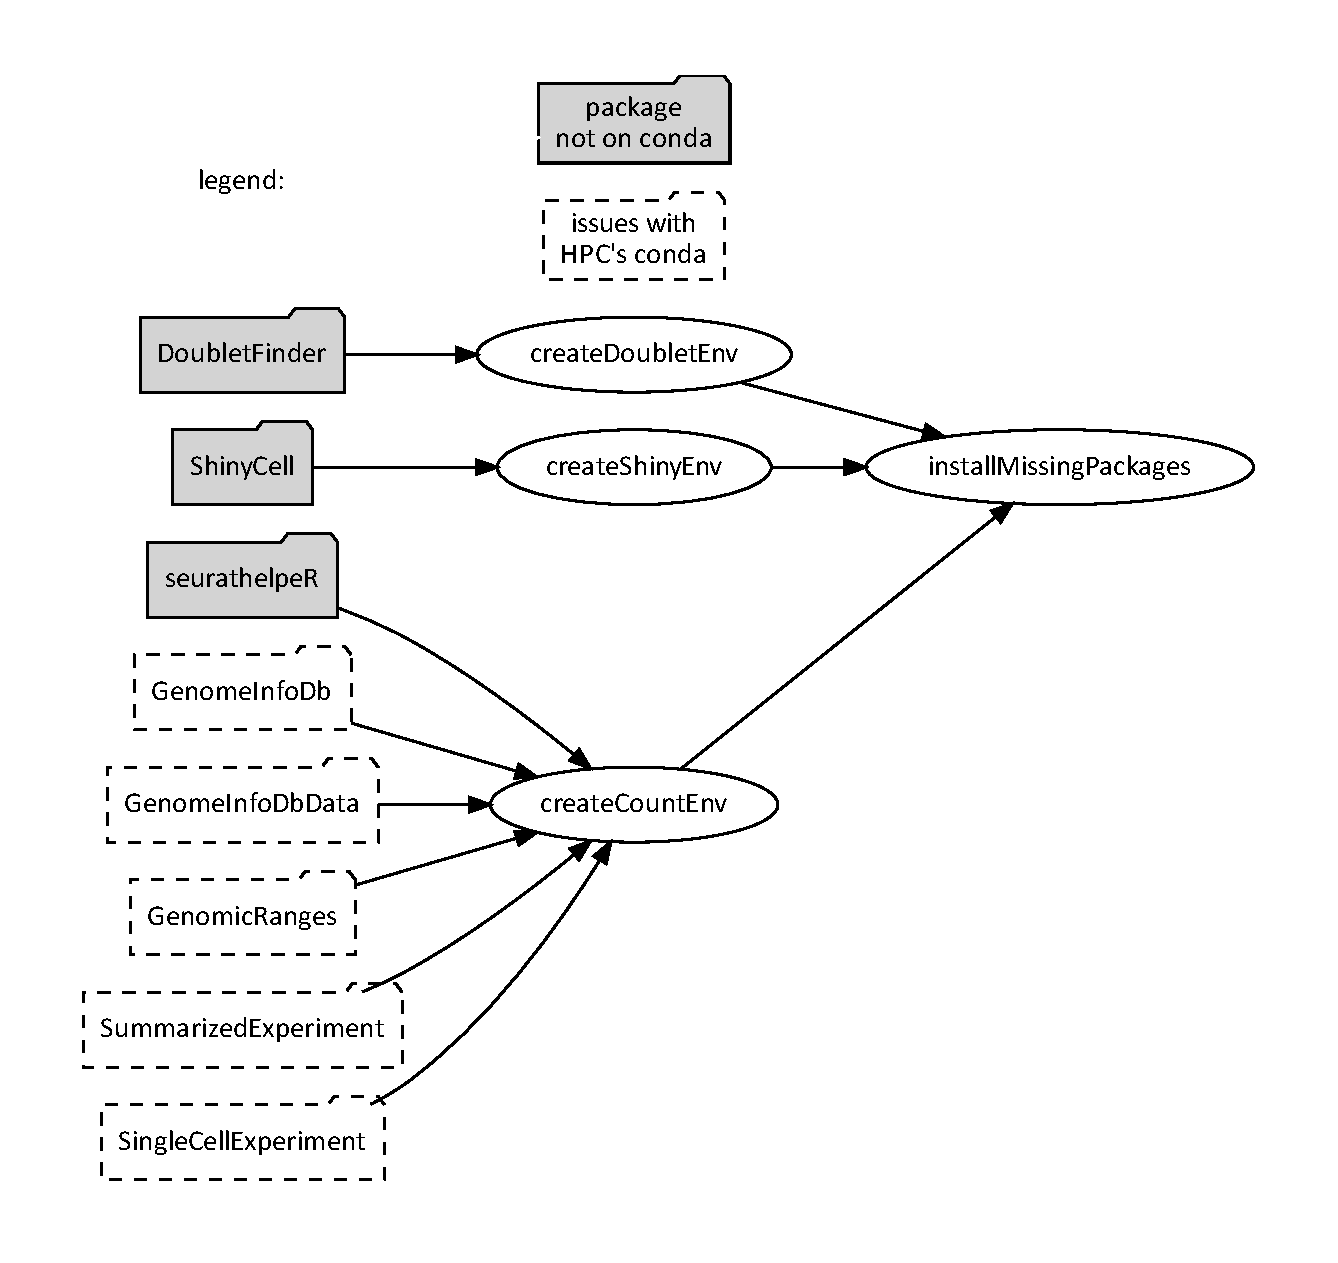
\includegraphics[width=1\textwidth]{figures/installRun.pdf}}
	\caption{How the installation run works.}
	\label{fig:installRun}
\end{figure}
 
\begin{figure}[h!]
	%\includesvg[width=\textwidth]{figures/pipelineRun.pdf}
	\centering
	\makebox[\textwidth][c]{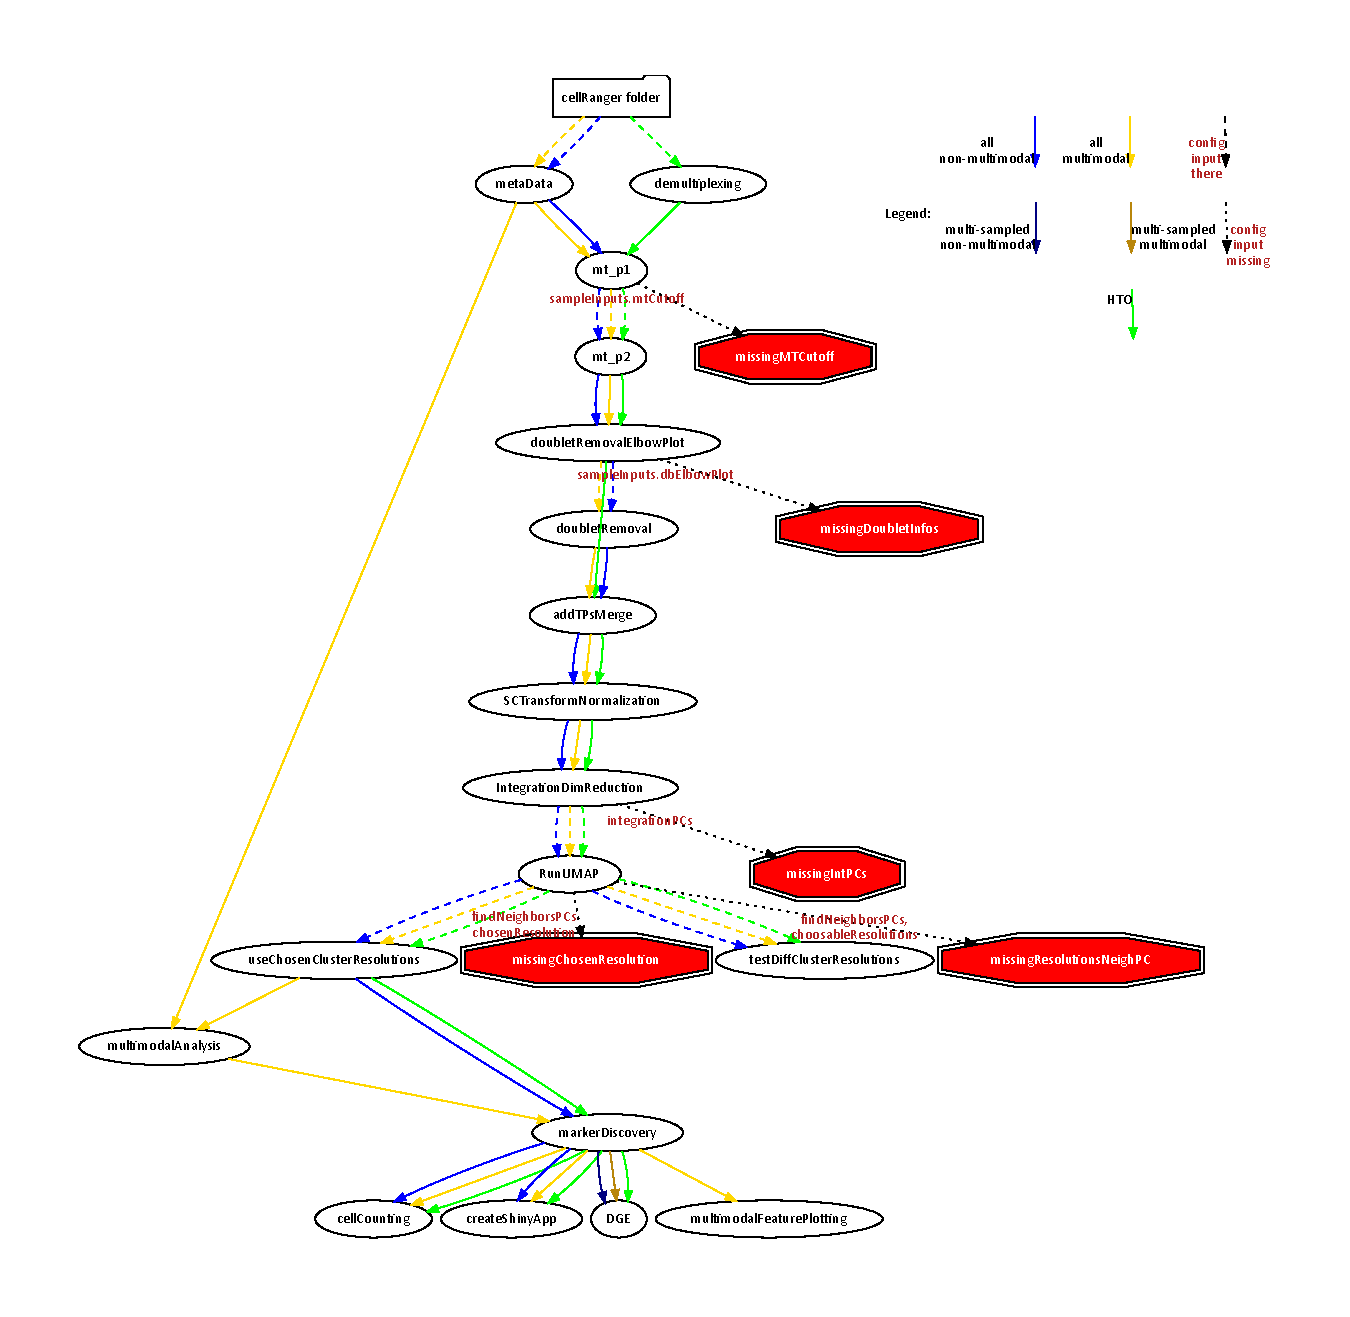
\includegraphics[width=1.55\textwidth]{figures/pipelineRun.pdf}}
	\caption{The three workflow ways.}
	\label{fig:pipelineRun}
\end{figure}

\subsection{metaData}
The metaData step is used for both non-multimodal and multimodal datasets though not for HTO. It reads the 10X Cellranger folder and transforms the dataset into a SeuratObject. It will then add the sample names to each sample and create an output for each sample respectively called \textbf{sample\_name}.metaData.rds. If the dataset had additional data like protein data it will create an additional output called \textbf{projectname}.rawData.rds.

\subsection{demultiplexing}
The demultiplexing step is for HTO datasets. Here too, the 10X Cellranger folder is read and transformed into a SeuratObject. The HTO data is added as an assay and the SeuratObject is demultiplexed. A scatter plot called \textbf{projectname}.HTOscatter.pdf. is created and then the doublets are removed. The sample name is then added to each sample and each sample is outputted as \textbf{sample\_name}.demux.rds.

\subsection{mt\_p1}
This step calculates the percentage of counts belonging to mitochondrial reads for each cell. It will then create violin plots called \textbf{sample\_name}.mt.before.pdf from which the user should determine at what percentage of mitochondrial reads the cells of a sample should be filtered. After this step a \textbf{\textit{MissingInputError}} will be thrown until the user enters a percentage for each sample into the "mtCutoff" slot in the config.yaml.

\subsection{mt\_p2}
After the percentages where entered into the config.yaml, this step will remove all cells that had a percentage of mitochondiral reads greater than the cutoff value. It will then create a \textbf{sample\_name}.mt.after.pdf plot for each sample for a before and after comparison.

\subsection{doubletRemovalElbowPlot}
For each sample this step performs SCT normalization and PCA before creating an elbow plot. The elbow plot is used to determine the "dbElbowPlot" in the config.yaml. The value describes the PCs/dimensions for the doublet removal. A \textbf{\textit{MissingInputError}} will be thrown until an value is entered for each sample.

\subsection{DoubletRemoval}
Only if not HTO, otherwise this step is skipped. Here DoubletFinder removes the doublets.

\subsection{addTPsMerge}
Here additional meta data from "otherMetaName" and "otherMetaData" is added to the respective samples as well as all possible combinations created from the two configs. E.g., if the dataset has condition and timepoint as meta data the combination condition.timepoint will be created. Afterwards all samples are combined into a single dataset again and outputted as \textbf{projectname}.preprocessedO.rds.

\subsection{SCTransformNormalization}
SCT normalization is performed for each sample in the dataset.

\subsection{IntegrationDimReduction}
If the dataset has multiple samples, Seurat's integration via anchors is performed followed by PCA. Otherwise only PCA is performed. Then the elbow plot \textbf{projectname}.integratedElbowPlot.pdf is created, so the user can choose the number of PCs for UMAP. A \textbf{\textit{MissingInputError}} will be thrown until the number of PCs us entered as "integrationPCs" in the config.

\subsection{RunUMAP}
UMAP with the number of PCs of "integrationPCs" from config is performed. The two plots \textbf{projectname}.umappedDimPlot.pdf and \textbf{projectname}.umappedElbowPlot.pdf are created. The elbow plot is used to find the number of PCs for "findNeighborsPCs" in config which describes the number of PCs used in Seurat's "FindNeighbors" function. Until a value is entered into the config, the \textbf{\textit{MissingInputError}} will be thrown. The error will also be thrown until "choosableResolutions" is filled out. More on that in the next subsection.

\subsection{testDiffClusterResolutions \& useChosenClusterResolution}
Next, clustering should be performed. Seurat controls the number of clusters with a "resolution" variable in the FindClusters function. A resolution below 1 gives less while a resolution above 1 gives more clusters. The step testDiffClusterResolutions is used to create multiple plots with different resolutions from "choosableResolutions" from the config if the user does not know what resolution is used. After choosing a resolution useChosenClusterResolution is perfomed for the actual clustering of the dataset using "chosenResolution" in the dataset.

\subsection{multimodalAnalysis}
This is only performed if the dataset is multimodal. Here, the additional data like protein data will be added to the dataset. However, currently only "Antibody Capture" can be added.

\subsection{markerDiscovery}
The dataset is normalized and scaled. Gene markers are found through the FindAllMarkers function of Seurat. These markers are written into two .CSV files in csv/.\\ \textbf{projectname}.compareGE\_inAll.markers.csv contains the output of FindAllMarkers while \textbf{projectname}.compareGE\_inAll.avgExpression.csv contains the output of AverageExpression.

\subsection{cellCounting}
For each condition or condition combination a bar plot is created containing the relative number of cells in a cluster grouped by condition type. If there are multiple samples error bars will be created describing the standard deviation.

\subsection{createShinyApp}
A shiny app for the dataset is created through ShinyCell.

\subsection{DGE}
For each condition (combination) differentially expressed genes are calculated by comparing each condition type in each cluster with each other and saved in .CSV files. If one condition has less than three cells compared to the other condition the comparison is skipped and noted in finishedDGE.txt. Only for multi-sampled dataset.

\subsection{multimodalFeaturePlotting}
For each feature in the extra assay a feature plot \textbf{feature}.adtFeatureProtein.pdf is created.
\newpage

\section{Setup config.yaml}
\label{section:config}
In this section, we describe how to fill out a config.yaml. A config.yaml gives the pipeline information on what kind of dataset it is processing and how it should be processed. Information on how to fill out a config.yaml is also in the configfiles/config\_example.yaml. In the table~\ref{tab:config} you can see each input with an explanation of what should be entered. If there is an X in the \textit{S} column then the input has to be filled out in the very beginning or the pipeline won't start.

\begin{tabular}{p{3.5cm} | p{9.5cm} | p{0.1cm}}
	\label{tab:config}
	Input & Description & S\\
	\hline
	HHU\_HPC & Is the pipeline run on the HHU HPC? Depending on whether the input is \textbf{true} or \textbf{false} the HHU\_HPC environments or the netAccess environments will be used. & X\\
	maxRAM & The maximal global RAM the pipeline is allowed to use. If unsure, just copy the value from config\_example.yaml. Even if that value is greater than the physical RAM, the 32 GB in config\_example.yaml should not be reached unless there are a few million cells in the dataset. & X\\
	workDirectory & the R work directory during the pipeline run. & X\\
	rawData & The directory containing the cellranger outputs which serves as this pipelines input. & X\\
	mtPattern & The pattern of mitochondrial reads in the dataset, e.g. "mt\^~". & X\\
	multimodal & Is this a multimodal dataset meaning does it contain protein data? \textbf{true} or \textbf{false}. & X\\
	multiSampled & Does this dataset contain more than one sample? \textbf{true} or \textbf{false}. & X\\
	HTO & Does this dataset use HTOs? \textbf{true} or \textbf{false}. & X\\
	numberOfCells & How many cells does this dataset contain? & X\\
	projectName & The name of the project. & X\\
	otherMetaName & Condition names for the meta data. E.g., [timepoint, donor, condition] & X\\
	choosableResolutions & List of resolution the user looks at before choosing one for clustering. In []. Resolution for Seurat's \textit{FindClusters}. & \\
	chosenResolution & The resolution chosen after taking a look at the "chosenResolutions". Resolution for Seurat's \textit{FindClusters}. & \\
	integrationPCs & The PCs for \textit{RunUMAP}. For choosing the PCs check the plot ending with ".integratedElbowPlot.pdf". & \\
	findNeighborsPCs & PCs used for the SNN-Graph in \textit{FindNeighbors}. For choosing PCs check the plot ending with ".umappedElbowPlot.pdf" & \\
	sampleInputs: & A collection of information about each sample. & X\\
\end{tabular}

\newpage

The values below have to be added to "sampleInputs" and has to be created for every sample. See configfiles/config\_example.yaml for an example.

\begin{tabular}{p{4cm} | p{9.5cm} | p{0.1cm}}
	Input & Description & S\\
	\hline
	name & The name of the sample. & X\\
	otherMetaData & The meta data type for condition name. Has to be in [] and in the same order as the names in "otherMetaData" in the table above. E.g., [day1, donorA, cancer] & X\\
	expectedPercentDoublets & Expected percent doublets. & X\\
	mtCutoff & Percentage cutoff chosen during the pipeline run. E.g. enter 10 if you want to remove all cells with more than 10\% mitochondrial counts. Check plots ending with "mt.before.pdf". & \\
	dbElbowPlot & PCs chosen from plots for \textit{RunUMAP} and \textit{doubletFinder\_v3} in DoubletRemoval. Check plots ending with ".ElbowPlot.pdf" & \\
\end{tabular}

\newpage

\section{Running the Pipeline}
\label{section:runPipeline}
Here different ways of running the pipeline are described. Important to note is that the pipeline will throw a \textbf{\textit{MissingInputError}} when an input value is missing in the config. Usually you need to take a look at plots created during the pipeline run to choose these input values correctly which is why the custom error exists. To interrupt the pipeline so the user can input a the value. However, the values can also be entered at the beginning of the run allowing for a single uninterrupted run.

If you have finished running the pipeline and wish to rerun the pipeline from a certain point onward, delete/rename the output from the step you want to rerun in the outputs folder and restart the pipeline.

First, move your 10X Cellranger Output folder into the data/ folder a config.yaml for you dataset, see section~\ref{section:config} for more.

\subsection{Simple Snakemake Command}
Install Anaconda or Miniconda and create a Snakemake environment. The Pipeline should work best with Snakemake 5.10.0 and might not work as well with higher versions of Snakemake. There are three packages not on conda that would be installed manually via a script through the install run, see~\ref{fig:installRun}. Download the following packages and move them into the dependencies/ folder.
\begin{itemize}
	\item https://github.com/chris-mcginnis-ucsf/DoubletFinder (as .zip)
	\item https://github.com/SGDDNB/ShinyCell (as .zip)
	\item https://github.com/genomics-kl/seurathelpeR (as .zip)
\end{itemize}
Next, switch to the scRAseq\_Pipeline/ folder in the terminal if you have not already. Change the HPC\_HHU input in the config.yaml to \textbf{false}. For the install run use the command:
\begin{center}
	snakemake -p -{}-cores 1 -{}-use-conda -{}-configfile path/to/config.yaml
\end{center}
After all packages are installed and use the following command for an actual run. 
\begin{center}
	snakemake -p -{}-cores \underline{X} -{}-use-conda -{}-configfile path/to/config.yaml
\end{center}
\textit{X} marks the number of cores you want to use. Cores can be used to perform multiple jobs at ones, e.g., if you have 6 samples you can choose 6 cores and the pipeline will process the 6 samples simultaneously until the samples are merged back into one dataset. In case of a Snakemake error during a run, Snakemake will lock the directory and you cannot run the pipeline again unless you run the following command to unlock the directory.
\begin{center}
	snakemake -p -{}-cores 1 -{}-use-conda -{}-configfile path/to/config.yaml -{}-unlock
\end{center}
The conda environments used here are in the netAccess folder. If you want to customize these environments more either change the envs in the netAccess folder or create a new folder and change the paths in the pipeline options, see section~\ref{section:pipeOptions}.


\subsection{Run on the HHU HPC}
First download the pipeline and put it into your scratch\_gs or project\_gs folder since a single run can create over 50 GB in outputs. Next, move you 10X Cellranger Output folder into the data/ folder. Now, download the following packages and move them into the dependencies folder:
\begin{itemize}
	\item https://github.com/chris-mcginnis-ucsf/DoubletFinder (as .zip)
	\item https://github.com/SGDDNB/ShinyCell (as .zip)
	\item https://github.com/genomics-kl/seurathelpeR (as .zip)
	\item https://bioconductor.org/packages/release/bioc/html/GenomeInfoDb.html (ver.1.30.0 as tar.gz)
	\item https://bioconductor.org/packages/release/data/annotation/html/GenomeInfoDbData.html (ver.1.2.7 as tar.gz)
	\item https://bioconductor.org/packages/release/bioc/html/GenomicRanges.html (ver.1.46.1 as tar.gz)
	\item https://bioconductor.org/packages/release/bioc/html/SummarizedExperiment.html (ver.1.24.0 as tar.gz)
	\item https://bioconductor.org/packages/release/bioc/html/SingleCellExperiment.html (ver.1.16.0 as tar.gz)
\end{itemize}
The versions are important for compatibility with the environment for the HPC. \textbf{Important} if you copy from the config\_example.yaml make sure to change the path of "projectDirectoryPath" to a path you have access to and change the HPC account an project in the snakemakeScripts/cluster/cluster.json to ones belonging to you.

Now log into the HPC via your terminal and create a screen with the command "screen -S screen\_name". This way you will not lose any progress if you were to lose your Internet connection for a moment and can reconnect to your screen via "screen -r screen\_name". If you want to process multiple datasets at once you can do that by creating multiple screens, e.g. "screen -S screen\_name1", "screen -S screen\_name2", etc. and follow the following instructions for each screen:
\begin{itemize}
	\item Connect to the snakemake-node via "ssh snakemake-node". \textbf{Do not start the pipeline in the login-node}
	\item "cd" to the folder containing the pipeline repository.
	\item Use the command "bash clusterExecution.sh /path/to/config.yaml" to start the pipeline.
	\item If the folder is locked ,use the command "bash resumePipeline.sh /path/to/config.yaml" to unlock the pipeline.
	\item The pipeline will process your dataset until a \textbf{\textit{MissingInputError}} error comes at interruption. Then it will throw the error until the necessary input is entered into the config.yaml unless you chose to fill out everything before starting the pipeline.
	\item Repeat the above step until the pipeline finished processing your dataset.
\end{itemize}
\textbf{IMPORTANT! There are a few common errors}. Mostly due to how the HPC works. For using the HPC you need to know \textit{in advance} how much RAM, walltime, nodes and cores you want to use. The pipeline will do this for you by approximating the RAM and walltime based on benchmarks made using certain dataset. However, there are times the pipeline will not approximate enough walltime and RAM for your dataset. In this case you can add additional walltime or RAM to the step that failed in the pipeline options, see section~\ref{section:pipeOptions}. 

To know if a pipeline error is caused by not using enough walltime or RAM see section~\ref{section:errorsAndImprovs}. If the error is neither a \textbf{\textit{MissingInputError}} error nor a walltime or RAM error there might be an issue with the pipeline. 
\vfill

\section{Additional Pipeline Options}
\label{section:pipeOptions}
In this section we describe a few additional options and functions that the pipeline has to offer.

\subsection{Walltime and RAM Approximation and Addition}
Currently, walltime and RAM are approximated using the needed time and RAM from previously benchmarked datasets. For each step it calculates $\frac{walltime}{numberOfCells}$ and $\frac{RAM}{numberOfCells}$ for each dataset and uses the greatest gradient as factor. This gradient is then multiplied by the number of the cells of the dataset you wish to process as an approximation. 

However, if the approximation is not enough for the HHU HPC you can increase it by adding a few GB RAM of a bit walltime in seconds into the snakemakeScripts/Pipelineoptions.py "addRAM" and "addTime" dictionaries for the steps that need it respectively. You can also add them at the very beginning if you do not trust the approximation.

\subsection{Benchmarking}
If you want to do some benchmarking to add to the approximation then you first need to remove the comments marks for the benchmarking in the Snakefile and increase execTimes to the number of times each step should be executed for each benchmark.

\subsection{Seurat and Snakemake Parallelization}
Seurat offers parallelization of certain functions by using the Future package. In snakemakeScripts/PipelineOptions.py you can increase the number of cores for certain steps to decrease the walltime. All steps that \textbf{do not} have the multicore functions are marked with an X.

The pipeline itself also offers some parallelization functions. In the beginning the dataset is split into its individual sample (e.g. split into each patient). These samples can be processed simultaneously and independently from each other. If you run the pipeline on the HHU HPC you do not need to do any extra steps for this parallelization.

If you do not run the pipeline on the HHU HPC, but via the snakemake command, you need to set X in the snakemake option "--cores X" to the maximum number of cores you want to use.

\begin{figure}[h!]
	%\includesvg[width=\textwidth]{figures/pipelineRun.pdf}
	\centering
	\makebox[\textwidth][c]{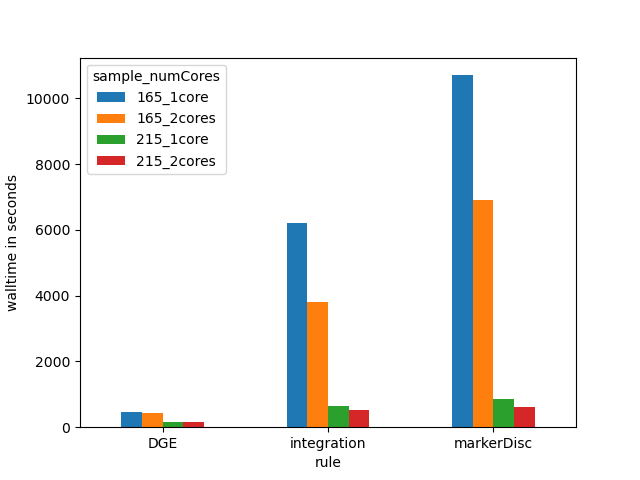
\includegraphics[width=1\textwidth]{figures/paraFutureBars.png}}
	\caption{Walltime reduction through parallelization with Seurat and Future.}
	\label{fig:parallelBars}
\end{figure}

\subsection{Conda Environments}
You can create your own folder with your own conda\_envs.yaml in the envs/ folder and change the environments in snakemakeScripts/PipelineOptions.py in the else case of the "setCondaEnv" function if you do not run the pipeline on the HHU HPC.

\newpage

\section{Possible Errors and Improvements}
\label{section:errorsAndImprovs}
In this section we discuss some common errors. How to fix them and places at which the pipeline can be improved.

\subsection{Common Errors and their Fixes}
As mentioned in previous sections there are a few intended and a few common errors that can occur in the pipeline. The table contains these errors and their fixes. These are mostly errors occurring in the HHU HPC

\begin{tabular}{p{3.5cm} | p{10cm}}
	Error & Fix\\
	\hline
	MissingInputError & Intentional error for interruption. Take a look at the error message on the terminal/in the logs and fill in the entry that is missing in the config.ymal.\\
	Not enough RAM & A HHU HPC error where not enough RAM was approximated. If you see in the logs that the error message contains "/bin/bash: line 1: \_\_\_\_ Killed" or something similar with "killed" then it is most likely this error. Add some additional GB RAM to the snakemakeScripts/PipelineOptions.py step that threw that error and restart the pipeline.\\
	Not enough walltime & A HHU HPC error where not enough Walltime was approximated. \textbf{The HPC does not throw an error message here}. If your terminal screen says that the job is still running, but myJAM says the job is not running anymore then the walltime ran out without finishing. Cancel the pipeline in the terminal, add some additional seconds to the walltime in snakemakeScripts/PipelineOptions.py to the step that threw the error and restart the pipeline.\\
	KeyError & If the pipeline throws a KeyError along with a name for an config.yaml entry. You might have wrote the name down incorrectly in your config.yaml\\
	Integer \& String errors & Be mindful of using the correct datatype in the config.yaml. E.g., if you want to name your project after a number, e.g. 215, then the number must be in "" otherwise the pipeline will read it as a number and not a word.\\
	command $\backslash$r not found & There might be an issue with the bash scripts since some of them were written on Windows or moved from Windows to Linux. To correct this issue use the command 'sed -i 's/$\backslash$r//g' filename.sh' where the filename is the bash script with the issue. 
\end{tabular}

\subsection{Conda and Package Issues}
Currently, a script is used to install the packages belonging to the dependencies folder. This is due to the package not being on conda. A fix for this would be if the packages would be added to bioconda which you can do yourself. However, to do so the packages need a tagged GitHub version release which only the creator of the used package can do.

Additionally, seuratHelper and DoubletFinder have Seurat version 3 compatibilities and are still working with Seurat version 4. This might change with version 5 though so it might be good to look for alternatives.

On the HHU HPC the conda module has issues with two of the Bioconductor packages in the dependencies folder. The other 3 are dependent on them, which is why the five have to be installed via the script on the HHU HPC. If the conda version where to be updated to a version above 4.6 then it might be possible to add these packages with these versions to the conda environments YAMLs and there would be no need to install them via the script anymore.

\subsection{Improvements for the Pipeline}
Currently, the pipeline only accepts "Antibody Capture" as additional assay for multimodal analysis. This could be more generalized to allow a greater variety of assays to be added.

Multicore parallelization with DoubletFinder is possible, but throws an error which states that 1 core did not deliver its processed data 50\% of the time. This could be correct.

The pipeline runs on Snakemake version 5.10.0. It should be adapted to higher versions of Snakemake for the future.

The naming of functions and variables in every script could be imrpoved.

The way the walltime and RAM are approximated could be improved by taking into account the size of the files and the number of cells per sample.

One could add different types of inputs instead of just the 10X Cellranger output folder.

The step addTPsMerge could be removed by adding the meta data in this step at the beginning and possibly skipping merge since SCTransformNormalization splits the dataset again.

\underline{Automatized cell annotation} could be added to the pipeline. To do so a script needs to be created and added to the Snakefile as a rule. If it should be between two certain steps, the output of the step that happens before needs to be the input of the annotation while the output of the annotation should become the input of the step that should follow in the Snakefile. An attempt for this had been made in the past, but it did not work out.

Seurat's Weighted Nearest Neighbor Analysis could be added.

There might be some other improvements that could be done which have not been found yet.
\newpage

	
	%	\newpage
	%	\addcontentsline{toc}{section}{List of Tables}
	%	\listoftables %optional
	%	
	%	\newpage
	%	\addcontentsline{toc}{section}{List of Figures}
	%	\listoffigures %optional
	%	
	%	\newpage
	%	\addcontentsline{toc}{section}{List of Abbreviations}
	%	\input{Abbrevs} %optional
\end{document}